% !TeX root = skripta-konstitutivni-vztahy.tex
% !TeX lastmodified = 2016-11-01

\subsection{Model Yeoh}\label{sec:yeoh}
\begin{itemize}
	\item YEOH (1993)
	\item vychází z Mooney-Rivlinovy formulace
	\item Yeoh dokázal, že celková energie napjatosti je více ovlivněna přírůstky $\frac{\partial W}{\partial I_1}$ než $\frac{\partial W}{\partial I_2}$ a~tedy je navržena řada v podobě:
	\begin{equation}
		W = C_{10} (I_1-3) + C_{20} (I_1-3)^2 + C_{30} (I_1-3)^3
	\end{equation}
	\item později bylo usouzeno, že se může vzít i vyšší počet členů
\end{itemize}
\begin{equation}
	W = \sum\limits_{i=1}^5 C_{i0} (I_1 - 3)^i
\end{equation}

\subsubsection{Důkaz}
Vychází se z~modelu Mooney-Rivlina (kapitola \ref{sec:mooney-rivlin})
\begin{equation}
	W = C_{10} (I_1-3) + C_{01} (I_2-3) + C_{20} (I_1-3)^2 + C_{11} (I_1-3) (I_2-3) + C_{30} (I_1-3)^3
\end{equation}
přičemž
\begin{equation*}
	\frac{\partial W}{\partial I_2} = C_{01} + C_{11} (I_2-3)
\end{equation*}
příspěvek je tedy nulový jen v případě, že $C_{01} = 0$ a~$C_{11} = 0$.

při dosazení zpět plyne původní forma konstitutivní rovnice ve tvaru:
\begin{equation}
	W = C_{10} (I_1-3) + C_{20} (I_1-3)^2 + C_{30} (I_1-3)^3
\end{equation}

\begin{figure}[H]
	\centering
	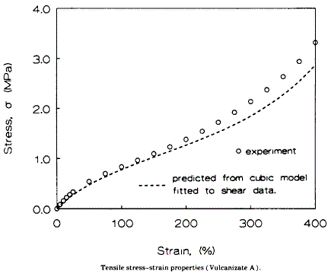
\includegraphics{yeoh-experiment-tah}
	\caption{Aproximace experimentu (tah) modelem Yeoh}
	\label{fig:yeoh-experiment-tah}
\end{figure}
\begin{figure}[H]
	\centering
	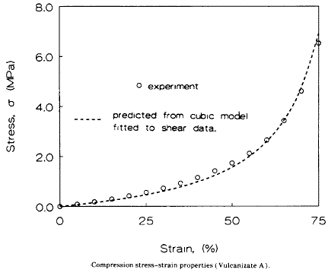
\includegraphics{yeoh-experiment-tlak}
	\caption{Aproximace experimentu (tlak) modelem Yeoh}
	\label{fig:yeoh-experiment-tlak}
\end{figure}